\begin{center}
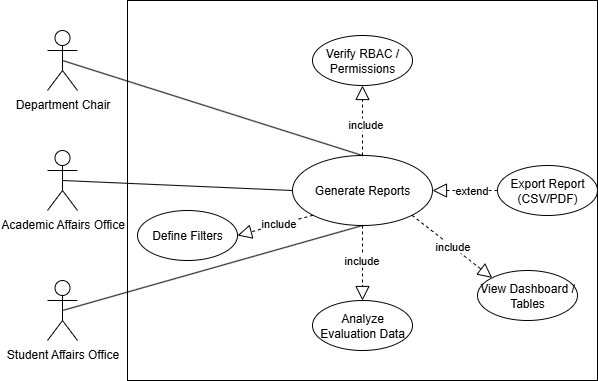
\includegraphics[width=0.9\linewidth]{images/UC-05.png}
\end{center}

\begin{center}
\textbf{Figure 6:}  Reporting and Analytics
\end{center}


\begin{table}[h!]
\centering
\begin{tabular}{|p{3cm}|p{11cm}|}
\hline
\textbf{Use-case ID} & UC-05a \\
\hline
\textbf{Use-case name} & Generate Departmental Report \\
\hline
\textbf{Use-case overview} & Department Chair generates a department-level report (attendance, performance, session counts) for academic monitoring and decisions. \\
\hline
\textbf{Actors} & Department Chair \\
\hline
\textbf{Preconditions} & 
1. Authenticated and authorized to view departmental reports. \newline
2. Sessions, feedback, and (if applicable) progress data exist. \newline
3. System is operational. \\
\hline
\textbf{Trigger} & Chair opens ``Reporting'' and selects ``Departmental Report''. \\
\hline
\textbf{Steps} & 
1. Set filters (term/date, program/department, tutor/cohort). \newline
2. System retrieves and analyzes metrics (attendance, performance, session counts). \newline
3. System displays tables/charts with data-source notes. \newline
4. Optional: Export CSV/PDF with metadata (generation time, filters, version); log action. \\
\hline
\textbf{Postconditions} & 
1. Departmental report displayed; optional file generated. \newline
2. Action recorded in the audit log. \\
\hline
\textbf{Alternative Flows} & 
1. Change filters/scope $\rightarrow$ system refreshes results. \\
\hline
\textbf{Exception Flow} & 
1. No data for selected criteria $\rightarrow$ show ``No data available for this selection.'' \newline
2. Export error (I/O or size) $\rightarrow$ suggest narrowing scope or retrying. \newline
3. Data source unavailable $\rightarrow$ show service notice; allow retry when available. \\
\hline
\end{tabular}
\caption{Use Case UC-05a: Generate Departmental Report}
\end{table}

\begin{table}[h!]
\centering
\begin{tabular}{|p{3cm}|p{11cm}|}
\hline
\textbf{Use-case ID} & UC-05b \\
\hline
\textbf{Use-case name} & View Tutor Workload Dashboard \\
\hline
\textbf{Use-case overview} & Academic Affairs views tutor workload and student demand to allocate resources effectively. \\
\hline
\textbf{Actors} & Academic Affairs Office \\
\hline
\textbf{Preconditions} & 
1. Authenticated and authorized for workload dashboards. \newline
2. Sessions/booking and feedback data exist. \newline
3. System is operational. \\
\hline
\textbf{Trigger} & Office opens ``Workload \& Demand'' dashboard. \\
\hline
\textbf{Steps} & 
1. Select filters (term/date, department/program). \newline
2. System aggregates tutor load and demand indicators. \newline
3. System displays dashboard (tables/charts, drill-down). \newline
4. Optional: Export CSV/PDF with metadata; log action. \\
\hline
\textbf{Postconditions} & 
1. Workload dashboard visible; optional export ready. \newline
2. Access recorded in the audit log. \\
\hline
\textbf{Alternative Flows} & 
1. Drill-down by tutor/program $\rightarrow$ refresh view. \\
\hline
\textbf{Exception Flow} & 
1. No data for selected criteria $\rightarrow$ show ``No data available for this selection.'' \newline
2. Export error (I/O or size) $\rightarrow$ suggest narrowing scope or retrying. \newline
3. Data source unavailable $\rightarrow$ show service notice; allow retry when available. \\
\hline
\end{tabular}
\caption{Use Case UC-05b: View Tutor Workload Dashboard}
\end{table}

\begin{table}[h!]
\centering
\begin{tabular}{|p{3cm}|p{11cm}|}
\hline
\textbf{Use-case ID} & UC-05c \\
\hline
\textbf{Use-case name} & Generate Participation Report \\
\hline
\textbf{Use-case overview} & Student Affairs generates participation reports for credit/scholarship consideration. \\
\hline
\textbf{Actors} & Student Affairs Office \\
\hline
\textbf{Preconditions} & 
1. Authenticated and authorized for participation reports. \newline
2. Sessions and attendance/feedback records exist. \newline
3. System is operational. \\
\hline
\textbf{Trigger} & Office selects ``Participation Report''. \\
\hline
\textbf{Steps} & 
1. Choose filters (term/date, cohort, program, thresholds). \newline
2. System compiles participation metrics and eligibility indicators. \newline
3. System displays results; Optional: export CSV/PDF with metadata; log action. \\
\hline
\textbf{Postconditions} & 
1. Participation report displayed; optional file generated. \newline
2. Action logged. \\
\hline
\textbf{Alternative Flows} & 
1. Adjust filters/criteria $\rightarrow$ refresh results. \\
\hline
\textbf{Exception Flow} & 
1. No data for selected criteria $\rightarrow$ show ``No data available for this selection.'' \newline
2. Export error (I/O or size) $\rightarrow$ suggest narrowing scope or retrying. \newline
3. Data source unavailable $\rightarrow$ show service notice; allow retry when available. \\
\hline
\end{tabular}
\caption{Use Case UC-05c: Generate Participation Report}
\end{table}
